%\documentclass{beamer}
%\usetheme{Warsaw}
%\usepackage{graphicx}


%\title[Short Title]{EE2227}
%\subtitle{Control System}
%\author{EE18BTECH11003}
%\date{February 12,2020}

%\begin{document}

%\begin{frame}
%\titlepage{}
%\end{frame}

%\begin{frame}{Question No 32(EC SECTION) 2019}

\begin{enumerate}[label=\thesection.\arabic*.,ref=\thesection.\theenumi]
\numberwithin{equation}{enumi}
\item
The block diagram of a system is illustrated in the figure shown, where X(s) is the input and Y(s) is the output. The transfer function

\begin{align}
 H(s)=\frac{Y(s)}{X(s)} 
\end{align}



%\begin{figure}
%\centering
%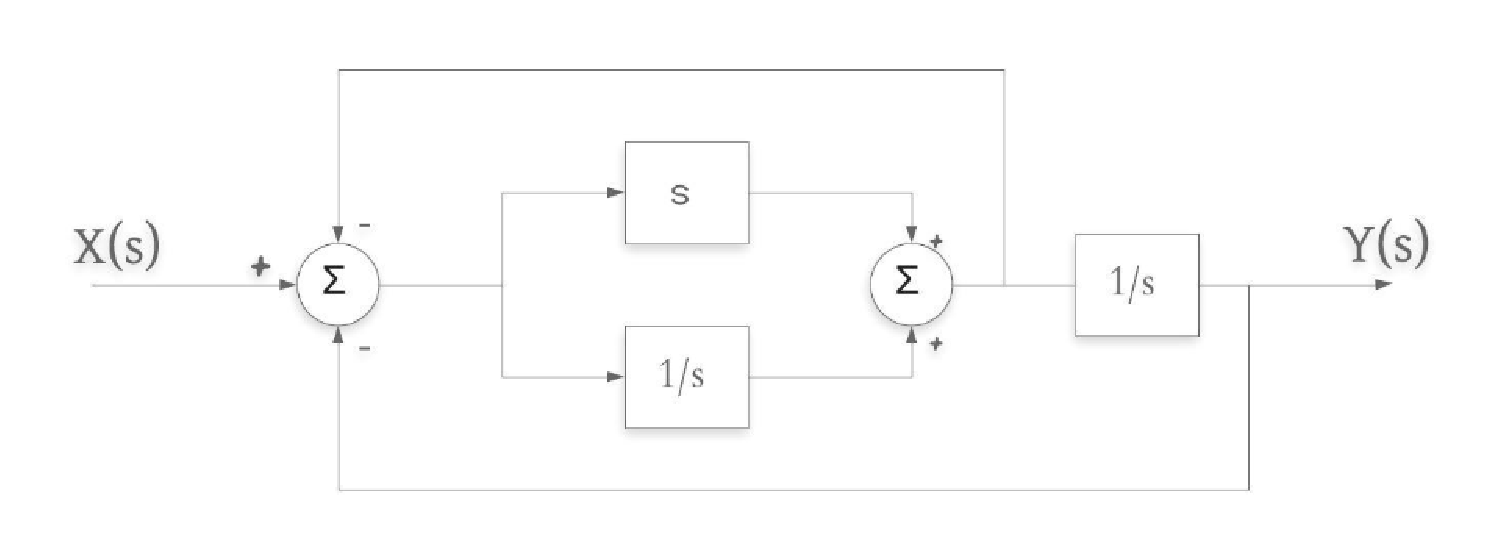
\includegraphics[width=0.8\textwidth]{./figs/pic1.eps}
%\caption{}
%\label{fig:sec_order}
%\end{figure}
\begin{figure}
\tikzset{
    block/.style = {draw, rectangle, 
        minimum height=1cm, 
        minimum width=2cm},
    input/.style = {coordinate,node distance=1cm},
    output/.style = {coordinate,node distance=4cm},
    arrow/.style={draw, -latex,node distance=2cm},
    pinstyle/.style = {pin edge={latex-, black,node distance=2cm}},
    sum/.style = {draw, circle, node distance=1cm}
    }
 \begin{center}
        \begin{tikzpicture}[auto, node distance=2.5cm,>=latex']
        \node [input, name=input] {};
        \node [sum, right of=input] (sum) {};
        \node [block, right of=sum] (controller) {$(1/s)$};
        \node [block, right of=controller] (plant) {$\sum$};
        \node [block, right of=plant] (summation) {$(1/s)$};
        \node [output, right of=summation] (output) {};
        \node [block, below of=plant] (feedback) {$1$};
        \node [block, above of=controller] (seed) {$s$};
        \node [block, right of=output] (leaf) {$Y(s)$};
        \node [block, above of=seed] (feed) {$1$};
        \draw [draw,->] (input) -- node {$X(s)$} (sum);
        \draw [->] (sum) -- node[name=p] {} (controller);
        \draw [->] (p) |- node [below,pos=1.69] {} (seed);
        \draw [->] (controller) -- node[name=c] {} (plant);
        \draw [<-] (sum) |- node [above,pos=0.79] {} (feed) ;
        \draw [<-] (plant) |- node  {} (seed);
        \draw [->] (plant) -- node [name=m] {}(summation);
        \draw [->] (summation) -- node[name=y] {} (leaf);
        \draw [->] (y) |- node [above,pos=0.79] {} (feedback) ;
        \draw [->] (feedback) -| node[pos=0.99] {$-$} 
        node [near end] {} (sum);
        
        \end{tikzpicture}
    \end{center}
\end{figure}

\begin{align}
 H(s)=\frac{s^2+1}{s^3+s^2+s+1}
\end{align}
\begin{align}
 H(s)=\frac{s^2+1}{s^3+2s^2+s+1}
\end{align}
\begin{align}
 H(s)=\frac{s^2+1}{s^2+s+1}
\end{align}
\begin{align}
 H(s)=\frac{s^2+1}{2s^2+1}
\end{align}

%\end{frame}

%\begin{frame}{Solution}

\solution 
\item Here we have two transfer function s and $\frac{1}{s}$ in parallel with a adder as shown in figure.
After solving these two parallel transfer function by just adding both of them we will get


%\begin{figure}
%\centering
%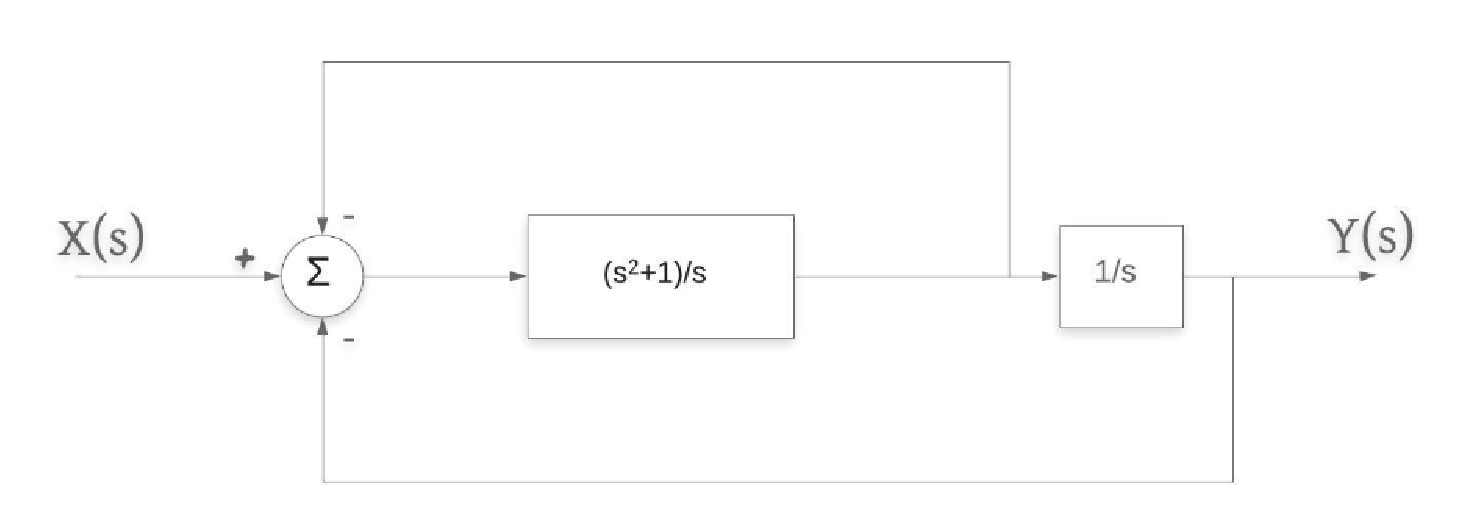
\includegraphics[width=0.8\textwidth]{./figs/pic2.eps}
%\caption{}
%\label{fig:sec_order}
%\end{figure}
%\end{frame}

\begin{figure}
\tikzset{
    block/.style = {draw, rectangle, 
        minimum height=1cm, 
        minimum width=2cm},
    input/.style = {coordinate,node distance=1cm},
    output/.style = {coordinate,node distance=4cm},
    arrow/.style={draw, -latex,node distance=2cm},
    pinstyle/.style = {pin edge={latex-, black,node distance=2cm}},
    sum/.style = {draw, circle, node distance=1cm}
    }
    \begin{center}
        \begin{tikzpicture}[auto, node distance=2.5cm,>=latex']
        \node [input, name=input] {};
        \node [sum, right of=input] (sum) {};
        \node [block, right of=sum] (controller) {$(s^2+1)/s$};
       % \node [block, right of=controller] (plant) {$\sum$};
        \node [block, right of=plant] (summation) {$(1/s)$};
        \node [output, right of=summation] (output) {};
        \node [block, below of=plant] (feedback) {$1$};
        %\node [block, above of=controller] (seed) {$s$};
        \node [block, right of=output] (leaf) {$Y(s)$};
        \node [block, above of=seed] (feed) {$1$};
        \draw [draw,->] (input) -- node {$X(s)$} (sum);
        \draw [->] (sum) -- node[name=p] {} (controller);
        %\draw [->] (p) |- node [below,pos=1.69] {} (seed);
        \draw [->] (controller) -- node[name=c] {} (summation);
        \draw [<-] (sum) |- node [above,pos=0.79] {} (feed) ;
        %\draw [<-] (plant) |- node  {} (seed);
        \draw [->] (plant) -- node [name=m] {}(summation);
        \draw [->] (summation) -- node[name=y] {} (leaf);
        \draw [->] (y) |- node [above,pos=0.79] {} (feedback) ;
        \draw [->] (feedback) -| node[pos=0.99] {$-$} 
        node [near end] {} (sum);
        
        \end{tikzpicture}
    \end{center}
\end{figure}

%\begin{frame}{Solution}
\item Now we will convert three input adder into two input adder as shown in figure given below.
%\begin{figure}
%\centering
%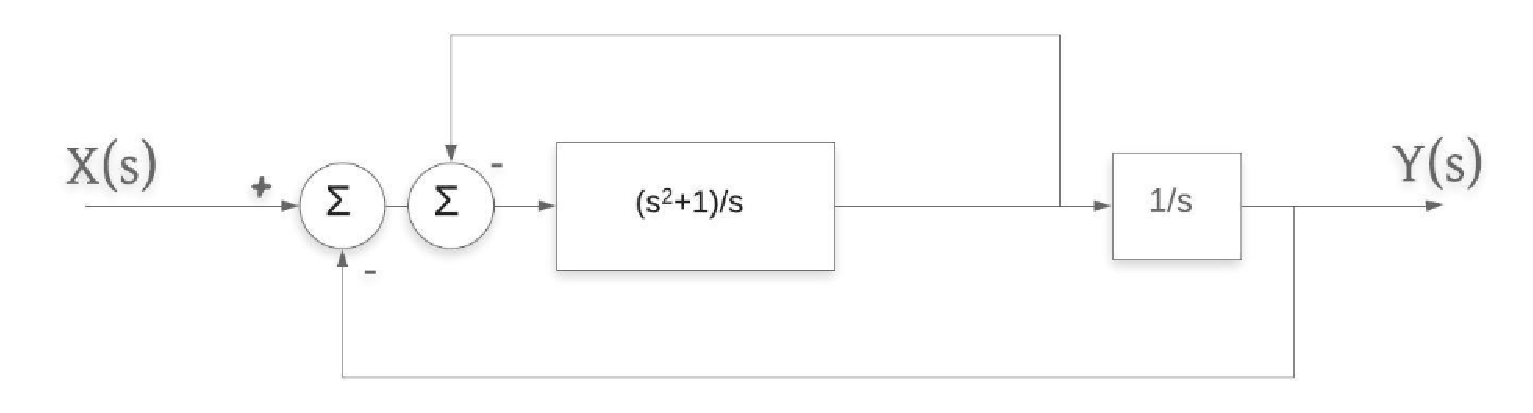
\includegraphics[width=0.8\textwidth]{./figs/pic3.eps}
%\caption{}
%\label{fig:sec_order}
%\end{figure}
%\end{frame}

%\begin{frame}{Solution}
\item Now we have Negative Unity Feedback System(NUFS) in closed loop transfer function.Let's say we have transfer function G(s) with Negative Unity Feedback System in closed loop then we will solve this by      

\begin{align}
 H(s)=\frac{G(s)}{1+G(s)}
\end{align}

%\\Here we have
%\begin{figure}
%\centering
%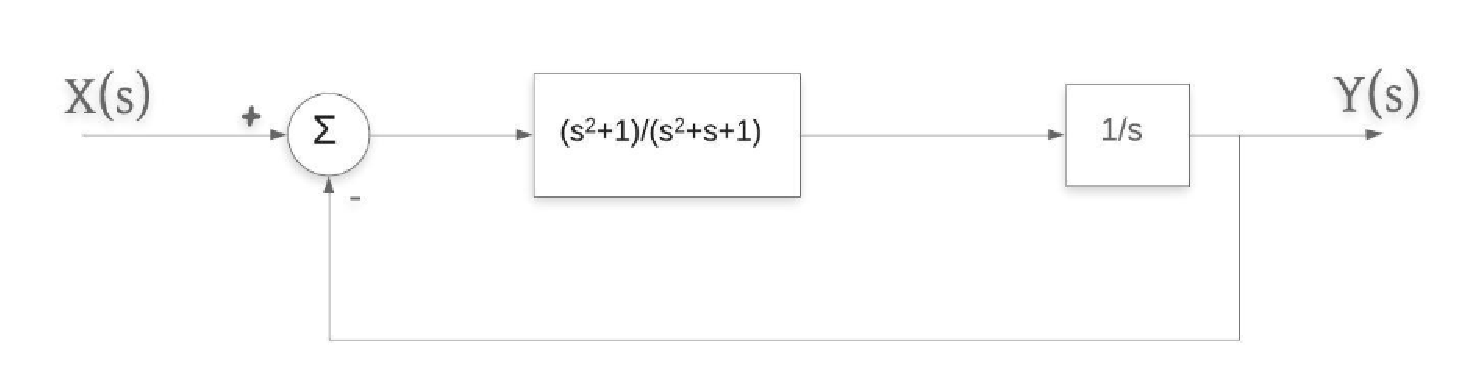
\includegraphics[width=0.8\textwidth]{./figs/pic4.eps}
%\caption{}
%\label{fig:sec_order}
%\end{figure}
%\end{frame}
\begin{figure}
\tikzset{
    block/.style = {draw, rectangle, 
        minimum height=1cm, 
        minimum width=2cm},
    input/.style = {coordinate,node distance=1cm},
    output/.style = {coordinate,node distance=4cm},
    arrow/.style={draw, -latex,node distance=2cm},
    pinstyle/.style = {pin edge={latex-, black,node distance=2cm}},
    sum/.style = {draw, circle, node distance=1cm}
    }
    \begin{center}
        \begin{tikzpicture}[auto, node distance=2.5cm,>=latex']
        \node [input, name=input] {};
        \node [sum, right of=input] (sum) {};
        \node [block, right of=sum] (controller) {$(s^2+1)/(s^2+s+1)$};
       % \node [block, right of=controller] (plant) {$\sum$};
        \node [block, right of=plant] (summation) {$(1/s)$};
        \node [output, right of=summation] (output) {};
        \node [block, below of=plant] (feedback) {$1$};
        %\node [block, above of=controller] (seed) {$s$};
        \node [block, right of=output] (leaf) {$Y(s)$};
        %\node [block, above of=seed] (feed) {$1$};
        \draw [draw,->] (input) -- node {$X(s)$} (sum);
        \draw [->] (sum) -- node[name=p] {} (controller);
        %\draw [->] (p) |- node [below,pos=1.69] {} (seed);
        \draw [->] (controller) -- node[name=c] {} (summation);
        %\draw [<-] (sum) |- node [above,pos=0.79] {} (feed) ;
        %\draw [<-] (plant) |- node  {} (seed);
        \draw [->] (plant) -- node [name=m] {}(summation);
        \draw [->] (summation) -- node[name=y] {} (leaf);
        \draw [->] (y) |- node [above,pos=0.79] {} (feedback) ;
        \draw [->] (feedback) -| node[pos=0.99] {$-$} 
        node [near end] {} (sum);
        
        \end{tikzpicture}
    \end{center}
    
\end{figure}

%\begin{frame}{Solution}
\item Here we have two transfer function in series 
%\begin{figure}
%\centering
%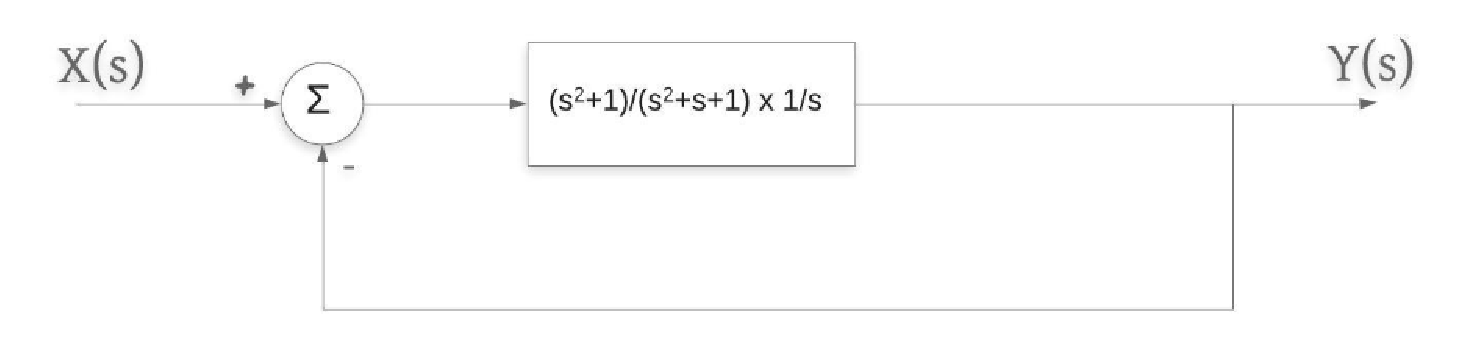
\includegraphics[width=0.8\textwidth]{./figs/pic5.eps}
%\caption{}
%\label{fig:sec_order}
%\end{figure}
%\end{frame}
\begin{figure}
\tikzset{
    block/.style = {draw, rectangle, 
        minimum height=1cm, 
        minimum width=2cm},
    input/.style = {coordinate,node distance=1cm},
    output/.style = {coordinate,node distance=4cm},
    arrow/.style={draw, -latex,node distance=2cm},
    pinstyle/.style = {pin edge={latex-, black,node distance=2cm}},
    sum/.style = {draw, circle, node distance=1cm}
    }
    \begin{center}
        \begin{tikzpicture}[auto, node distance=2.5cm,>=latex']
        \node [input, name=input] {};
        \node [sum, right of=input] (sum) {};
        \node [block, right of=sum] (controller) {$(s^2+1)/(s^3+s^2+s)$};
       % \node [block, right of=controller] (plant) {$\sum$};
        %\node [block, right of=plant] (summation) {$(1/s)$};
        \node [output, right of=summation] (output) {};
        \node [block, below of=plant] (feedback) {$1$};
        %\node [block, above of=controller] (seed) {$s$};
        \node [block, right of=output] (leaf) {$Y(s)$};
        %\node [block, above of=seed] (feed) {$1$};
        \draw [draw,->] (input) -- node {$X(s)$} (sum);
        \draw [->] (sum) -- node[name=p] {} (controller);
        %\draw [->] (p) |- node [below,pos=1.69] {} (seed);
        \draw [->] (controller) -- node[name=c] {} (output);
        %\draw [<-] (sum) |- node [above,pos=0.79] {} (feed) ;
        %\draw [<-] (plant) |- node  {} (seed);
        \draw [->] (plant) -- node [name=m] {}(summation);
        \draw [->] (summation) -- node[name=y] {} (leaf);
        \draw [->] (y) |- node [above,pos=0.79] {} (feedback) ;
        \draw [->] (feedback) -| node[pos=0.99] {$-$} 
        node [near end] {} (sum);
        
        \end{tikzpicture}
    \end{center}
   
\end{figure}


%\begin{frame}{Solution}
\item Now we have one more transfer function with negative unity feedback.

%\begin{figure}
%\centering
%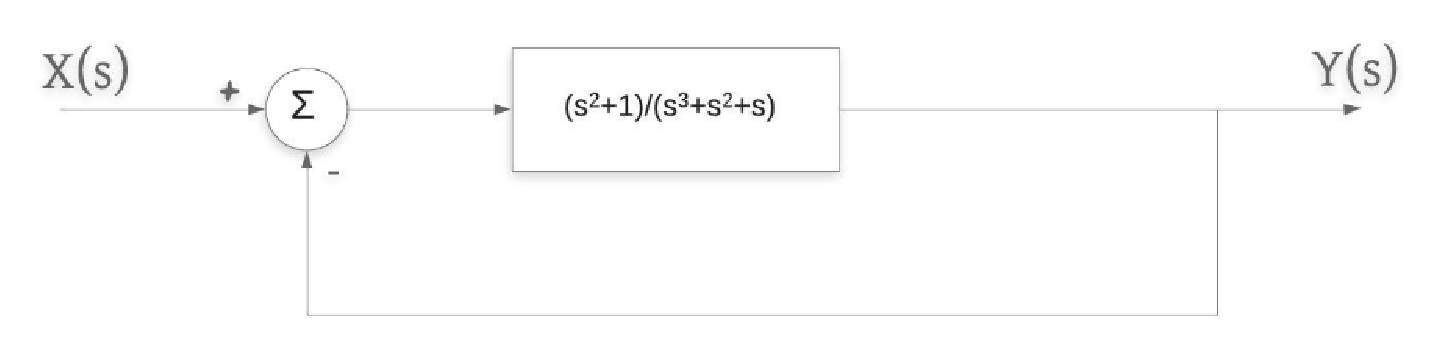
\includegraphics[width=0.8\textwidth]{./figs/pic6.eps}
%\caption{}
%\label{fig:sec_order}
%\end{figure}
\begin{figure}
\tikzset{
    block/.style = {draw, rectangle, 
        minimum height=1cm, 
        minimum width=2cm},
    input/.style = {coordinate,node distance=1cm},
    output/.style = {coordinate,node distance=4cm},
    arrow/.style={draw, -latex,node distance=2cm},
    pinstyle/.style = {pin edge={latex-, black,node distance=2cm}},
    sum/.style = {draw, circle, node distance=1cm}
    }
    \begin{center}
        \begin{tikzpicture}[auto, node distance=2.5cm,>=latex']
        \node [input, name=input] {};
        \node [sum, right of=input] (sum) {};
        \node [block, right of=sum] (controller) {$(s^2+1)/(s^3+2s^2+s+1)$};
       % \node [block, right of=controller] (plant) {$\sum$};
        %\node [block, right of=plant] (summation) {$(1/s)$};
        \node [output, right of=summation] (output) {};
       % \node [block, below of=plant] (feedback) {$1$};
        %\node [block, above of=controller] (seed) {$s$};
        \node [block, right of=output] (leaf) {$Y(s)$};
        %\node [block, above of=seed] (feed) {$1$};
        \draw [draw,->] (input) -- node {$X(s)$} (sum);
        \draw [->] (sum) -- node[name=p] {} (controller);
        %\draw [->] (p) |- node [below,pos=1.69] {} (seed);
        \draw [->] (controller) -- node[name=c] {} (output);
        %\draw [<-] (sum) |- node [above,pos=0.79] {} (feed) ;
        %\draw [<-] (plant) |- node  {} (seed);
        \draw [->] (plant) -- node [name=m] {}(summation);
        \draw [->] (summation) -- node[name=y] {} (leaf);
        %\draw [->] (y) |- node [above,pos=0.79] {} (feedback) ;
       % \draw [->] (feedback) -| node[pos=0.99] {$-$} 
        node [near end] {} (sum);
        
        \end{tikzpicture}
    \end{center}
    
\end{figure}

\item Again we will solve this then we will get
%\begin{figure}
%\centering
%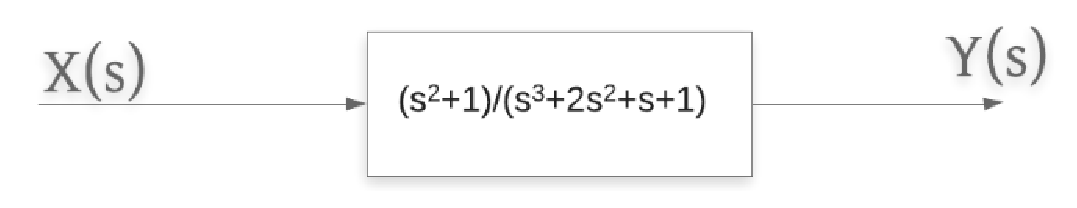
\includegraphics[width=0.8\textwidth]{./figs/pic8.eps}
%\caption{}
%\label{fig:sec_order}
%\end{figure}
%\end{frame}
%\begin{frame}{Solution}
%Now\\
\begin{align}
X(s)(\frac{s^2+1}{s^3+2s^2+s+1})=Y(s)
\end{align}

\begin{align}
\frac{Y(s)}{X(s)}=\frac{s^2+1}{s^3+2s^2+s+1}
\end{align}

\item The correct option is (B)

%\end{frame}
%\end{document}
\end{enumerate}